\documentclass[11pt]{article}

\usepackage{amsfonts}
\usepackage{fancyvrb}
\usepackage{url}
\usepackage{graphicx}
\usepackage{caption}
\usepackage{subcaption}
\usepackage{dsfont}

\setlength{\oddsidemargin}{0in}
\setlength{\evensidemargin}{0in}
\setlength{\textwidth}{6.5in}
\setlength{\topmargin}{0in}
\setlength{\headsep}{0.5in}
\setlength{\textheight}{8.5in}
\setcounter{page}{1}
%\pagestyle{empty}
%\hbadness=10000

\begin{document}
\huge
\noindent
{Discrete Optimization Assignment:}
\vspace{0.25cm}

\noindent
{\bf Facility Location}
\normalsize


\section{Problem Statement}

In this assignment you will design an algorithm to solve a problem faced by distribution companies, {\em The Facility Location Problem}. A distribution company uses bulk storage facilities to provide goods to many different customers.  The goal of this problem is to determine which facilities will be the most cost effective for serving the customers.  The complexity of the problem comes from the fact that each facility has different costs and storage capabilities.\footnote{Hint: The facility location problem is closely related to the warehouse location problem discussed in the lectures.} 

%\begin{figure}[h]
%        \centering
%        \begin{subfigure}[b]{8.0cm}%{0.3\textwidth}
%                \centering
%                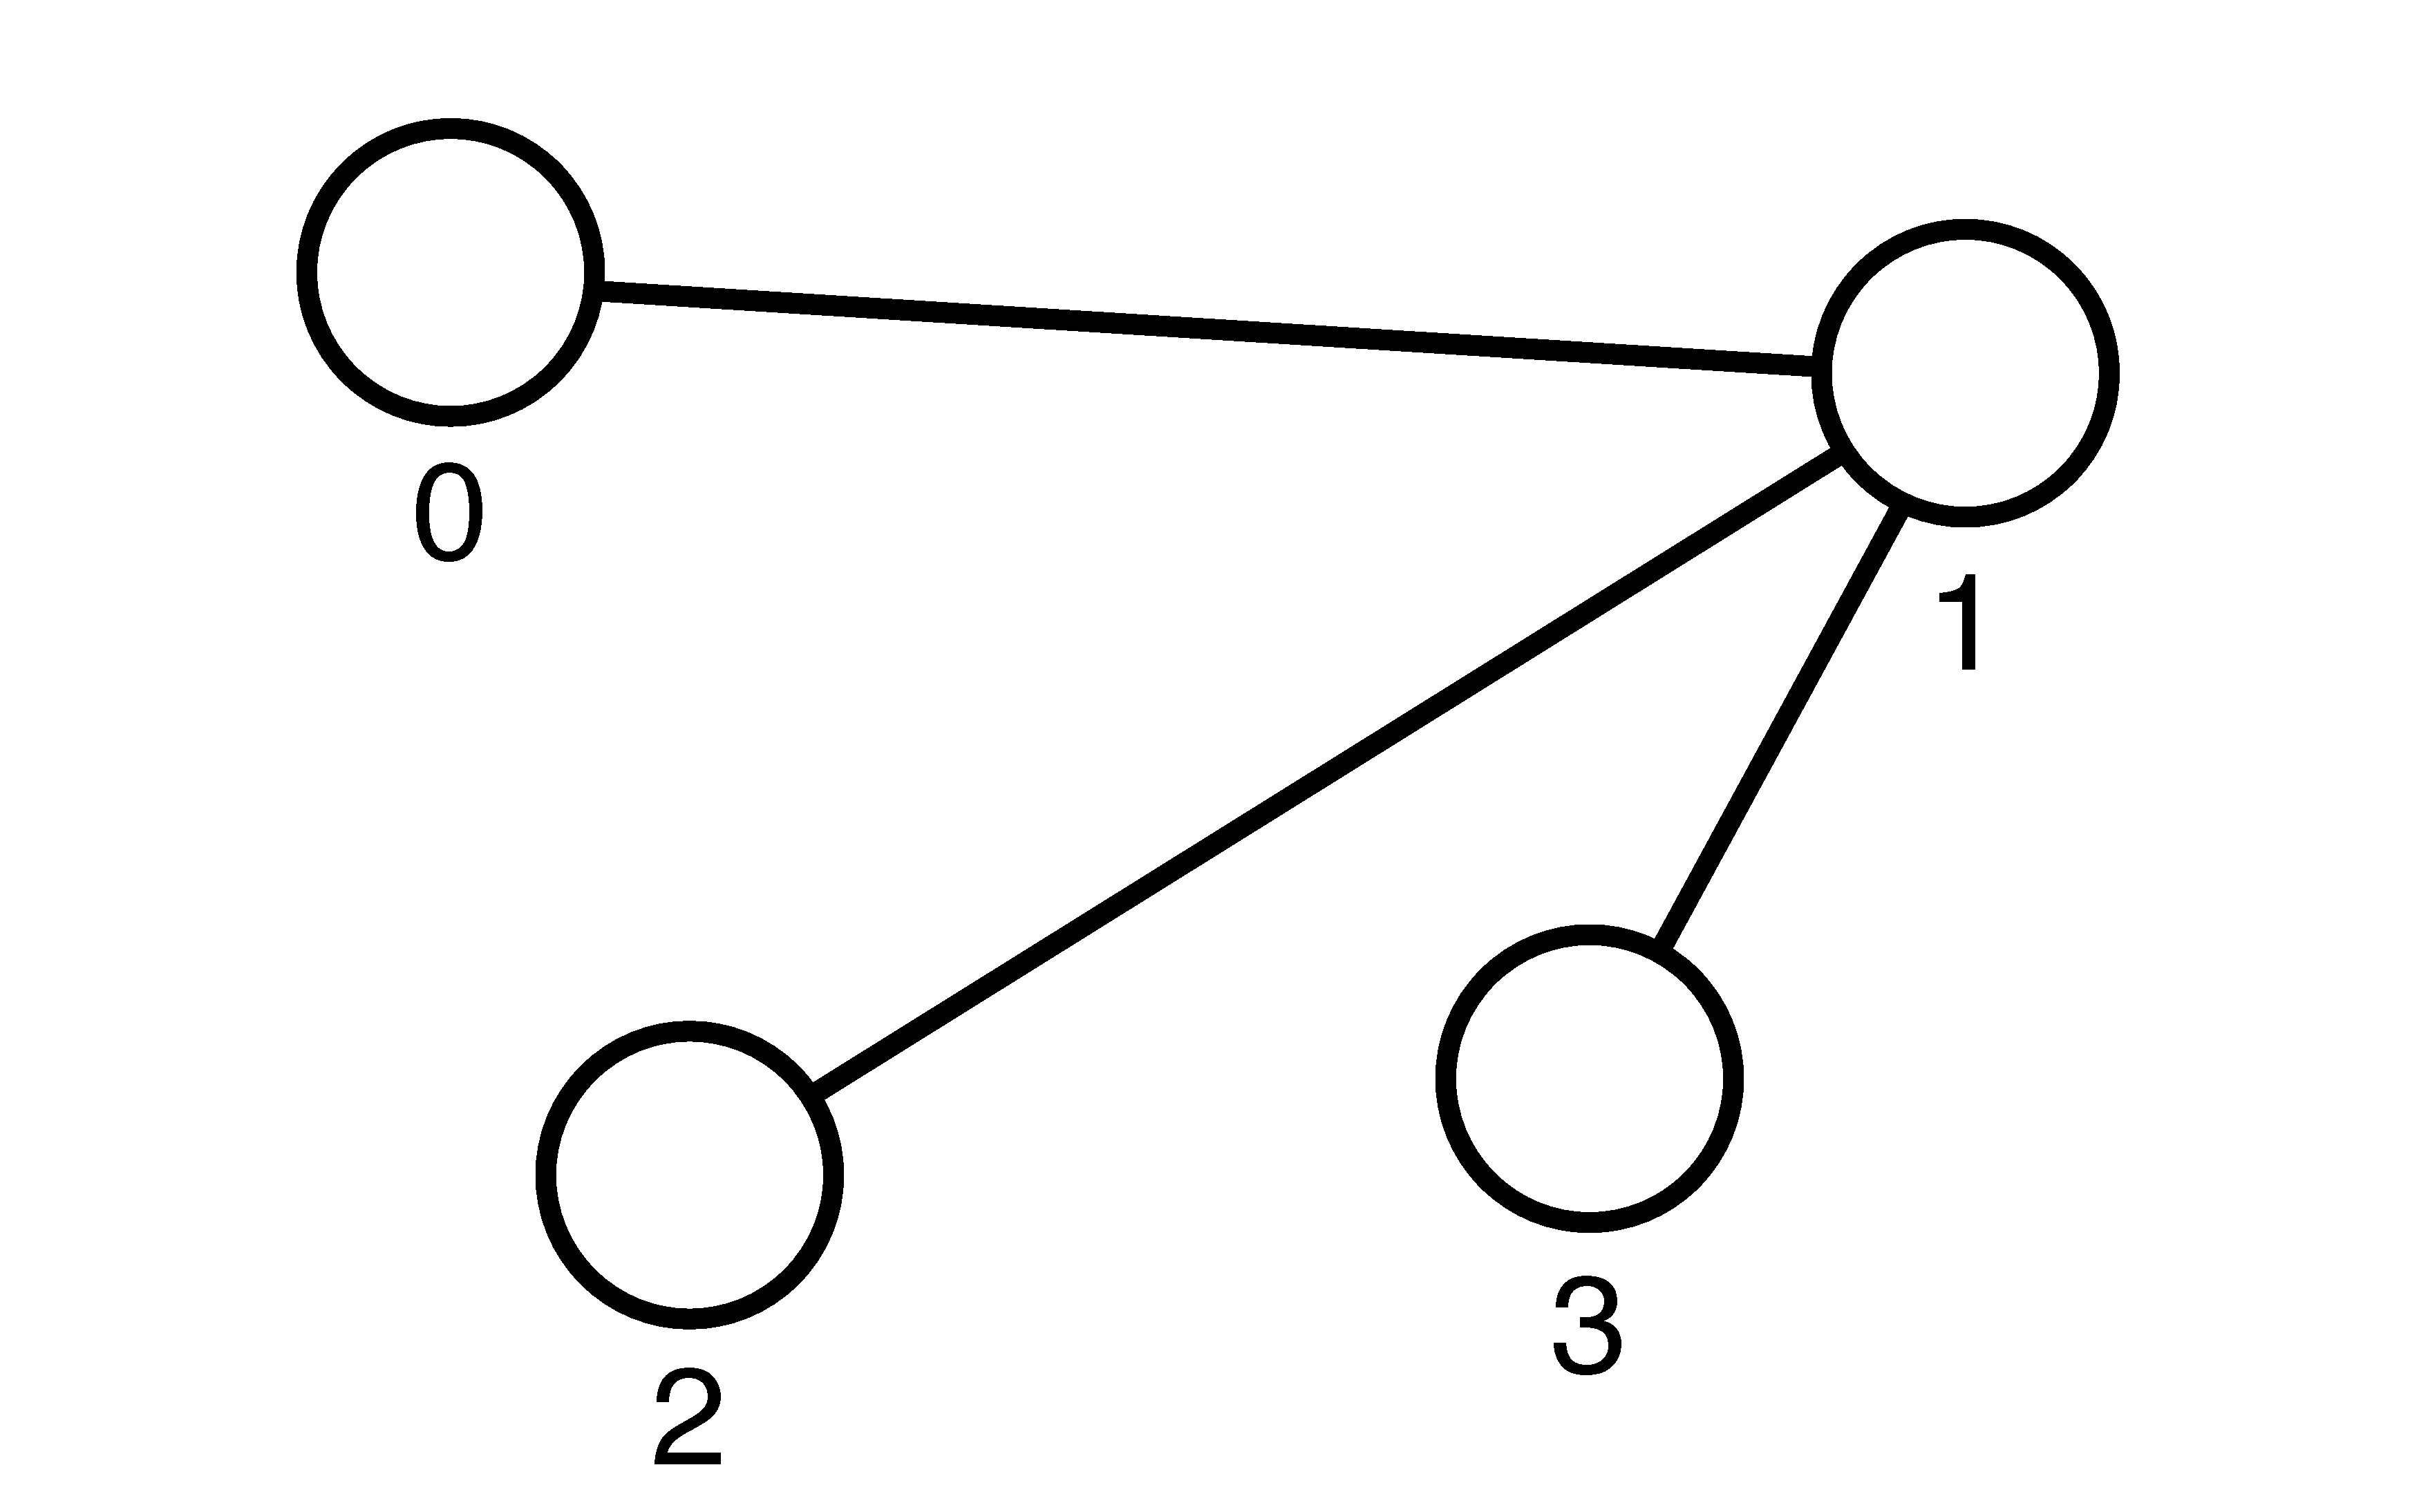
\includegraphics[width=8cm]{figures/coloring_1.pdf}
%                \caption{A graph.}
%                \label{fig:graph:input}
%        \end{subfigure}%
%        ~ %add desired spacing between images, e. g. ~, \quad, \qquad etc.
%          %(or a blank line to force the subfigure onto a new line)
%        \begin{subfigure}[b]{8.0cm}
%                \centering
%                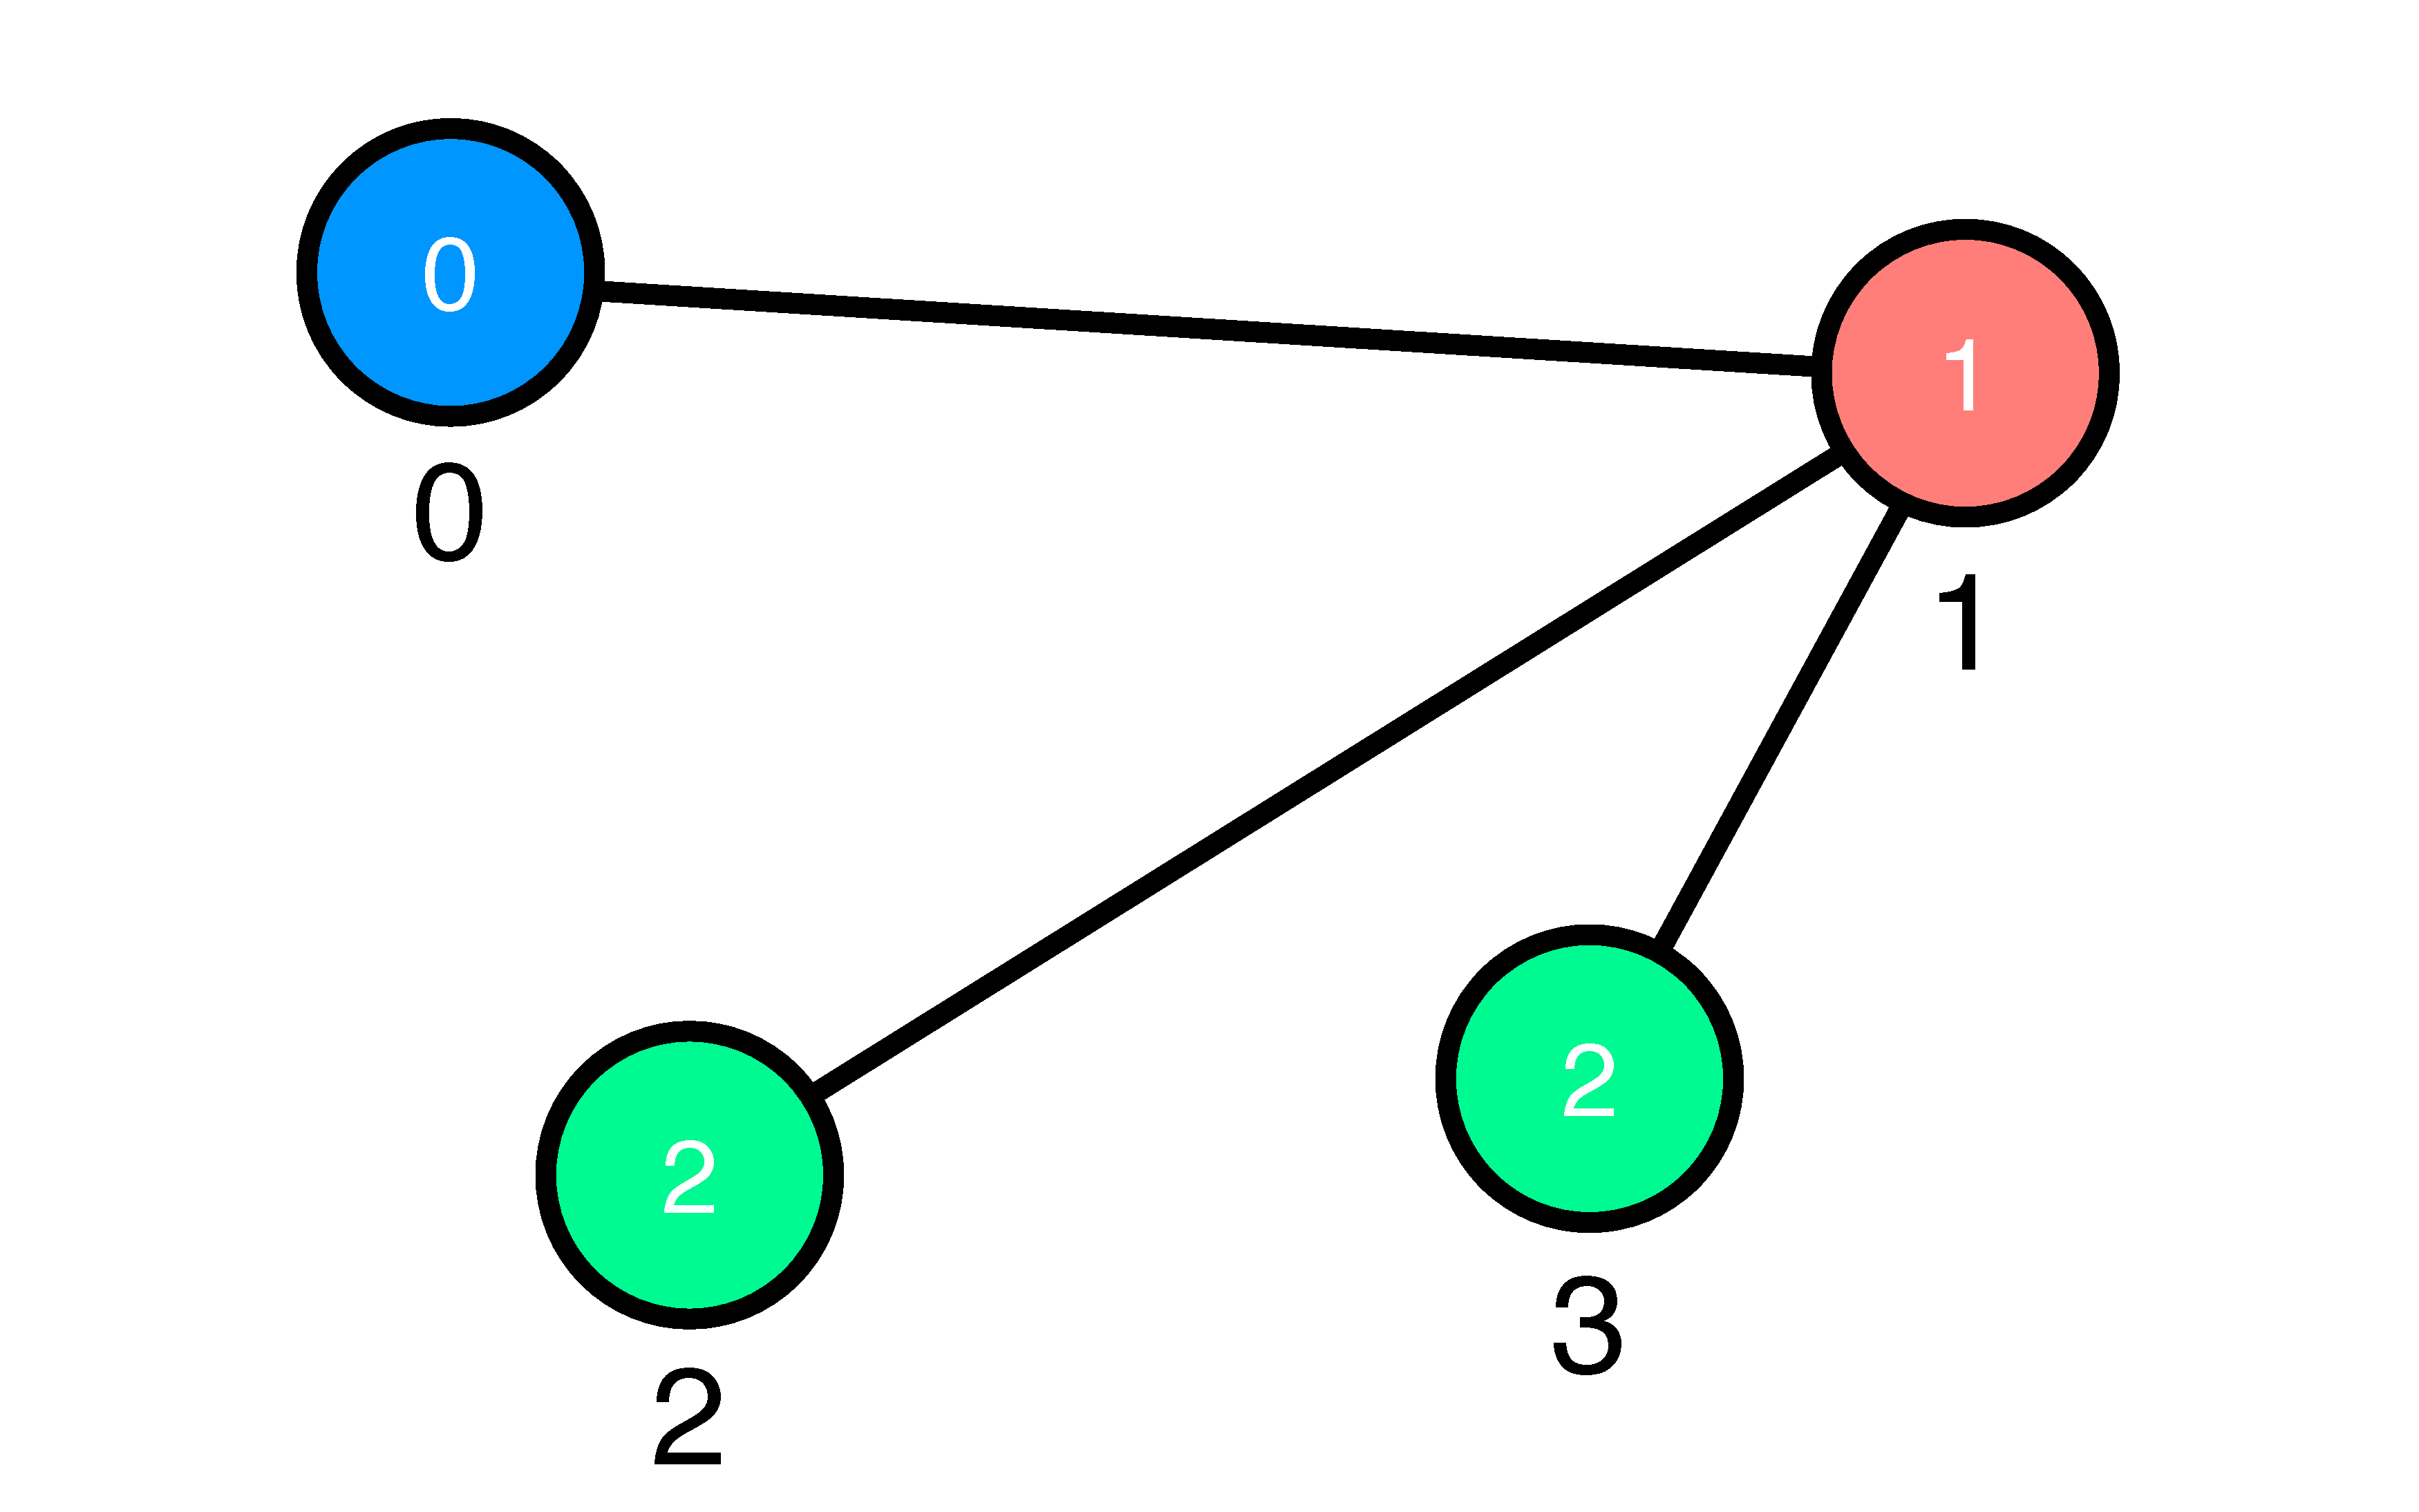
\includegraphics[width=8cm]{figures/coloring_2.pdf}
%                \caption{A three-coloring of the graph.}
%                \label{fig:graph:coloring}
%        \end{subfigure}
%        \caption{A Graph Coloring Example}\label{fig:graph}
%\end{figure}

\section{Assignment}

Write an algorithm to solve the facility location problem.  The problem is mathematically formulated in the following way:  there are $N = 0 \ldots n-1$ facilities to choose from and $M = n \ldots n+m-1$ customers that need to be served.  Each facility, ${\it f} \in N$ has a setup cost $s_{\it f}$ and a capacity $cap_{\it f}$.  Each customer, $c \in M$, has a demand $d_c$.  Both the facilities and customers are located in a Euclidian space, $\langle x_i,y_i \rangle \; i \in N \cup M$.  The cost to deliver goods to a particular customer $c$ from a facility ${\it f}$ is the Euclidean distance between two locations, ${\it dist}({\it f},c)$.\footnote{${\it dist}(i,j) = \sqrt{(x_{i} - x_{j})^2 + (y_{i} - y_{j})^2}$}  Lastly, all customers must be served by exactly 1 facility.  Let $a_f$ be a set variable denoting the customers assigned to facility $f$.  Then the facility location problem is formalized as the following optimization problem:
$$
\begin{array}{ll}
\mbox{minimize:} & \displaystyle \sum_{f \in N} \left( (|a_{\it f}| > 0) s_{\it f} + \sum_{c \in a_{\it f}} {\it dist}({\it f},c) \right) \\
\mbox{subject to:} & \\
     & \displaystyle \sum_{c \in a_{\it f}}  d_c \leq cap_{\it f} \;\;\; ({\it f} \in N)\\
     & \displaystyle \sum_{{\it f} \in N}  (c \in a_{\it f}) = 1 \;\;\; (c \in M) 
\end{array}
$$

\clearpage
\section{Data Format Specification}

The input consists of $|N| + |M| + 1$ lines.  The first line contains two numbers, $|N|$ followed by $|M|$.
The first line is followed by $|N|$ lines, where each line encodes the facility's setup cost $s_{\it f}$, capacity $cap_{\it f}$, and the location $x_{\it f}, y_{\it f}$.  The remaining $|M|$ lines capture the customer information, where each line encodes the customer's demand, $d_c$, and location $x_c, y_c$.

\vspace{0.2cm}
\noindent
Input Format
\vspace{-0.2cm}
\begin{Verbatim}[frame=single]
|N| |M|
s_0 cap_0 x_0 y_0
s_1 cap_1 x_1 y_1
...
s_|N|-1 cap_|N|-1 x_|N|-1 y_|N|-1
d_|N| x_|N| y_|N|
d_|N|+1 x_|N|+1 y_|N|+1
...
d_|N|+|M|-1  x_|N|+|M|-1 y_|N|+|M|-1
\end{Verbatim}
%
The output has two lines.  The first line contains two values: $obj$ and $opt$.  $obj$ is the cost of the customer to facility assignment (i.e. the objective value) as a real number.  $opt$ should be $1$ if your algorithm proved optimality and $0$ otherwise.  The next line is a list of $|M|$ values in $N$ -- this is the mapping of customers to facilities.

\vspace{0.2cm}
\noindent
Output Format
\vspace{-0.2cm}
\begin{Verbatim}[frame=single]
obj opt
c_0 c_1 c_2 ... c_|M|-1
\end{Verbatim}
%
%It is essential that the value order in the solution output matches the value order of the input.  Otherwise the grader will misinterpret the output.

\clearpage
\paragraph{Examples}
%\vspace{0.1cm}
%\noindent
%(based on Figure \ref{fig:graph})

\vspace{0.2cm}
\noindent
Input Example
\vspace{-0.2cm}
\begin{Verbatim}[frame=single]
 3 4 
 100 100 1065.0 1065.0
 100 100 1062.0 1062.0 
 100 500 0.0 0.0 
 50 1397.0 1397.0
 50 1398.0 1398.0 
 75 1399.0 1399.0 
 75 586.0 586.0
\end{Verbatim}

\vspace{0.2cm}
\noindent
Output Example
\vspace{-0.2cm}
\begin{Verbatim}[frame=single]
2550.013 0
1 1 0 2
\end{Verbatim}
%
This output represents the assignment of customers to facilities, $a_0 = \{2\}, a_1 = \{0,1\}, a_2 = \{3\}$.  That is, customers 0 and 1 are assigned to facility 1, customer 2 is assigned to facility 0, and customers 3 is assigned to facility 2.

\section{Instructions}

Edit \texttt{solver.py} and modify the \texttt{solve\_it(input\_data)} function to solve the optimization problem described above.  The function argument, \texttt{input\_data}, contains the problem data in the format described above.  The return value of \texttt{solve\_it} is a solution to the problem in the output format described above.  Your \texttt{solve\_it} implementation can be tested with the command, 
\[ 
\texttt{python ./solver.py ./data/<inputFileName>} 
\] 
You should limit the \texttt{solve\_it} method to terminate within 5 hours, otherwise the submission will not be eligible for full credit.  You may choose to implement your solver directly in python or modify the \texttt{solve\_it} function to call an external application.

%We use \texttt{stdout} for output.
%Output to other stream will be ignored (you may want to send runtime information to \texttt{stderr}). Your submission will be tested on a department linux machine. If your algorithm is a standalone program, please name it \texttt{nr},
%otherwise, please specify the compilation procedure,
%it is appreciated if you also provide a script that follows the above format to run the program.

\paragraph{Resources}
You will find several  facility location problem instances in the \texttt{data} directory provided with the handout.

%An example output file, \texttt{blabla.out}, is also provided.

%\section{Remarks}

\paragraph{Handin}
Run \texttt{submit.py} with the command, \texttt{python ./submit.py}.  Follow the instructions to apply your  \texttt{solve\_it} method on the various assignment parts.  You can submit multiple times and your grade will be the best of all submissions.  However, it may take several minutes before your assignment is graded; please be patient.  You can track the status of your submission on the {\em feedback} section of the assignment website.


\paragraph{Grading}
Infeasible solutions (i.e. those that do not conform to the output format or violate problem constraints) will receive 0 points.  Feasible solutions will receive at least 3 points.  Feasible solutions passing a low quality bar will receive at least 7 points and solutions meeting a high quality bar will receive all 10 points.  The grading feedback indicates how much your solution must improve to receive a higher grade.


\paragraph{Collaboration Rules} 

In all assignments we encourage collaboration and the exchange of ideas on the discussion forums.  However, please refrain from the following:
\begin{enumerate}
\item Posting code or pseudo-code related to the assignments.
\item Using code which is not your own.
\item Posting or sharing problem solutions.
\end{enumerate}
Discussion of solution quality (i.e. objective value) and algorithm performance (i.e. run time) is allowed and the assignment leader board is designed to encourage such discussions.


%\paragraph{Questions} Please contact the class GTA Carleton (cjc@cs.brown.edu).

\paragraph{Warnings} 

\begin{enumerate}
\item It is recommended you do not modify the \texttt{data} directory.  Modifying the files in the data directory risks
making your assignment submissions incorrect.
\item You cannot rename the \texttt{solver.py} file or the \texttt{solve\_it()} method.
\item Be careful when using global variables in your implementation.  The \texttt{solve\_it()} method will be run repeatedly and it is your job to clear the global data between runs.
\item \texttt{solver.py} must remain in the same directory as \texttt{submit.py}.
\end{enumerate}


%\paragraph{Hint} 
%The optimal value for  \texttt{data/gc\_1000\_5} is near $85$.
 
\section{Technical Requirements}

You will need to have python 2.7.x or 3.5.x installed on your system (installation instructions, \\ \texttt{\url{http://www.python.org/downloads/}}).


\end{document}




